\documentclass[11pt, a4paper, titlepage]{scrartcl}

\usepackage[utf8x]{inputenc}
\usepackage[frenchb]{babel}
\usepackage[T1]{fontenc}
\usepackage{graphicx}
\usepackage{hyperref}
\usepackage{float}

%\renewcommand{\familydefault}{\sfdefault}
%\usepackage[top = 2.54cm, bottom = 2.54cm, left=2.5cm, right=2.5cm]{geometry}

\titlehead{\centering
\includegraphics[width=\textwidth]{images/logo}}
\title{Projet Data Mining}
\author{Pierre \textsc{Turpin}, Jean-Marie \textsc{Comets}}
\date{\today}

\begin{document}

\maketitle
\tableofcontents
\newpage

Au vu des nombreux problèmes de "scaling" que nous pouvions rencontrer
avec le jeu de données prévu, l'intégralité de ce rapport repose sur
l'analyse d'un échantillon fixé des données, soit 5 000 streams.

\section{Caractérisation du flux vidéo}

% TODO qualitatif : localisations des joueurs
% TODO qualitative : mettre graphique evolution (nombre de vues, durées)
\begin{figure}[h]
    \centering
    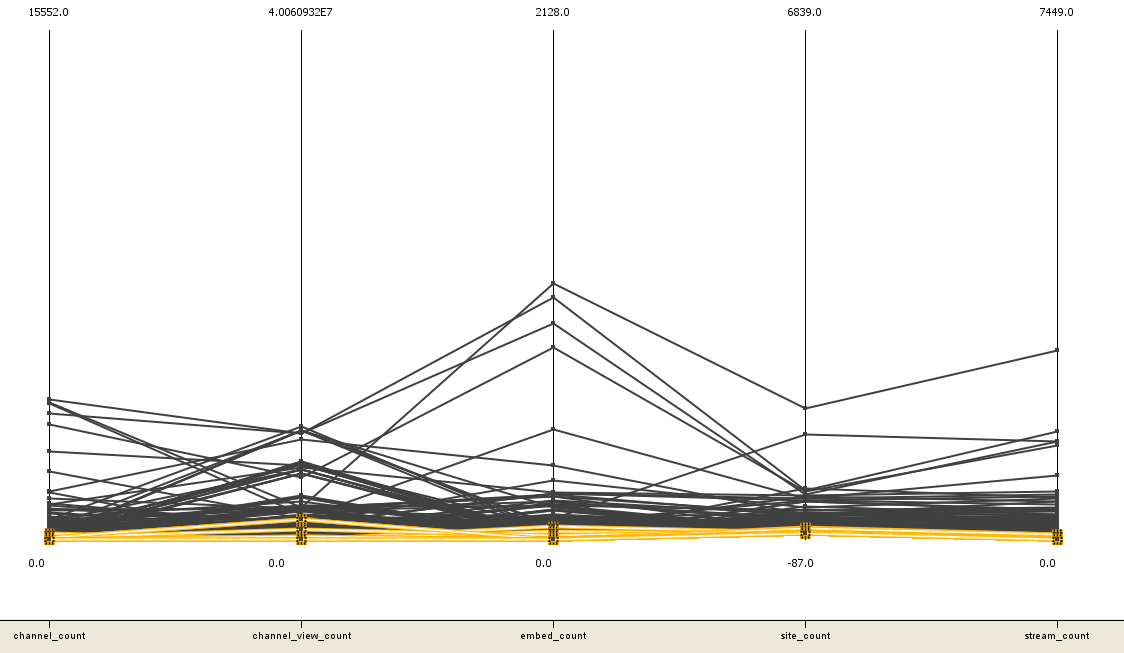
\includegraphics[width=\textwidth]{images/embed_enabled_influence}
    \caption{}
\end{figure}

\begin{figure}[h]
    \centering
    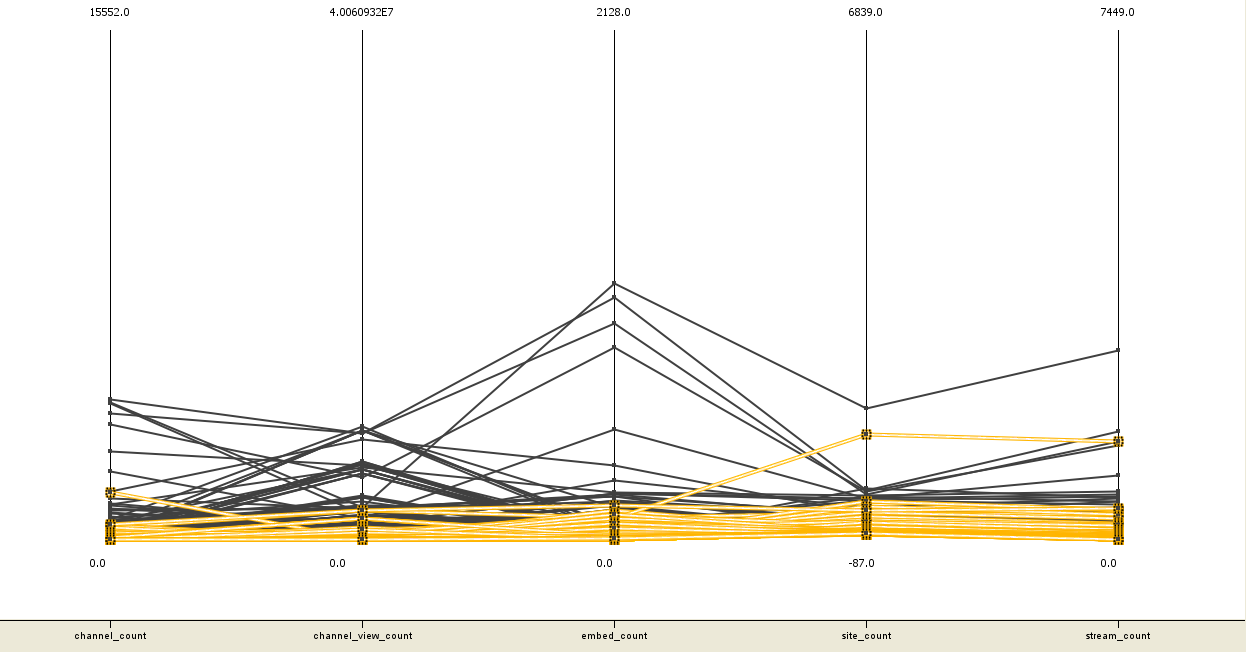
\includegraphics[width=\textwidth]{images/featured_influence}
    \caption{}
\end{figure}

\begin{figure}[h]
    \centering
    
\includegraphics[width=\textwidth]{images/logo}
    \caption{}
\end{figure}

\begin{figure}[h]
    \centering
    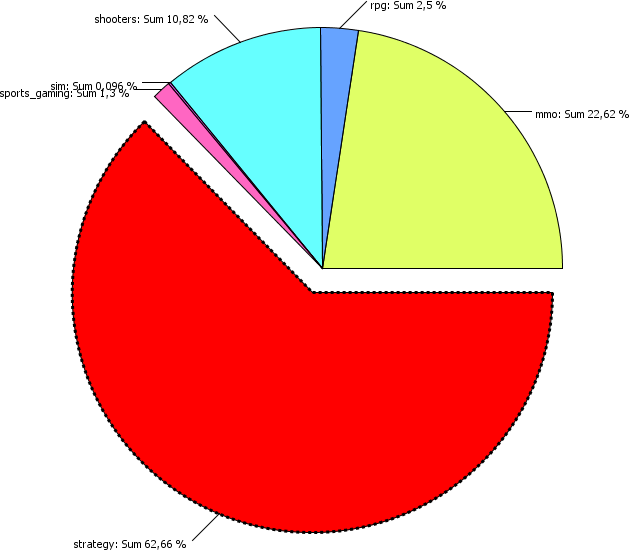
\includegraphics[width=\textwidth]{images/main_categories}
    \caption{}
\end{figure}

\begin{figure}[h]
    \centering
    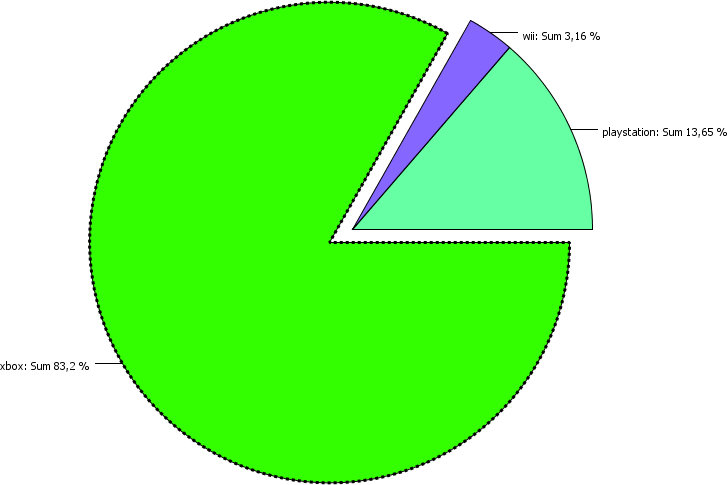
\includegraphics[width=\textwidth]{images/main_consoles}
    \caption{}
\end{figure}

\begin{figure}[h]
    \centering
    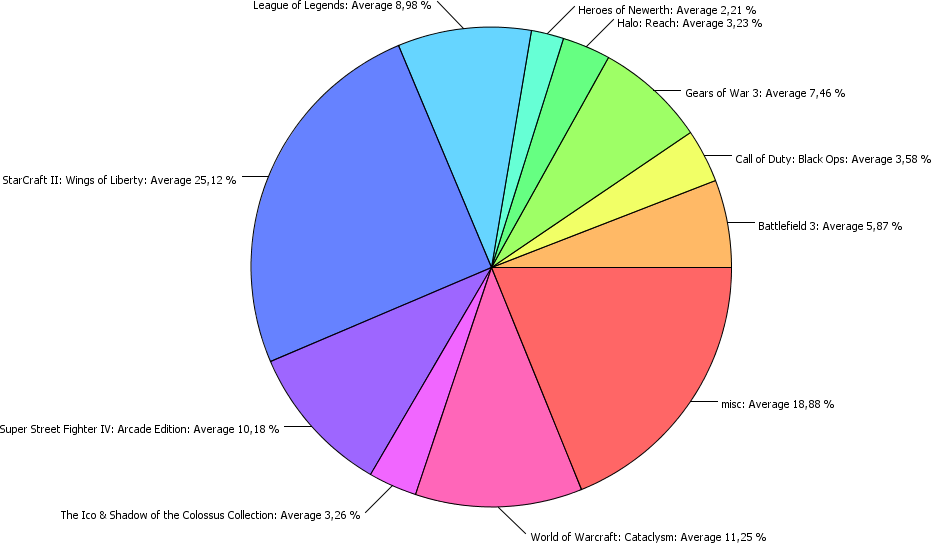
\includegraphics[width=\textwidth]{images/main_games}
    \caption{}
\end{figure}

\begin{figure}[h]
    \centering
    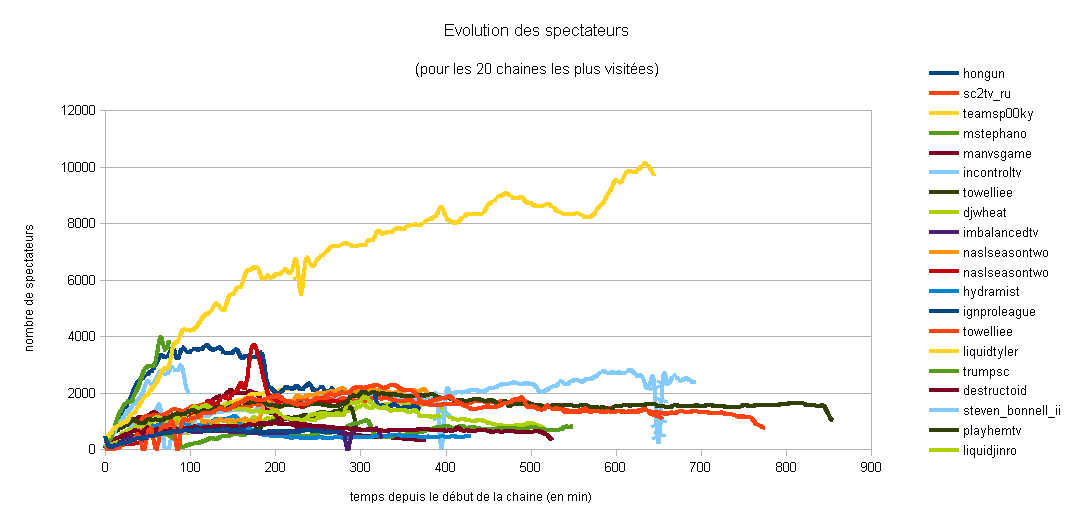
\includegraphics[width=\textwidth]{images/top_20_view_evolutions}
    \caption{}
\end{figure}

\section{Prédiction de l'audience d'un flux}

% TODO

\section{Classement des "meilleurs" joueurs}

% TODO classement par tableau/graphe

\end{document}
